\section{The groups on the archive}\label{sec:structure}

With the chosen values, $\delta=2$~min and $q=0.1$, 21.7\% of the paraglider flights and 6.9\% of
the hang-glider flights fly in a group at some point, in 17\,169 episodes (Table~\ref{tab:q}).
This section describes those groups: their sizes and durations, how they change, and where in the
flight and when in the day they form. Section~\ref{sec:group-structure} asks what holds them
together. Bands are 5--95\% of 200 draws of the dependency blocks, or of the dates where the
captions say so.

\subsection{Sizes and durations}\label{sec:sizes}

A configuration is a group with fixed members; it ends when a member joins or leaves. Its
duration runs from its start to its end, and its participants are its members at once. An episode
is a chain of configurations; its duration runs from the start of its first configuration to the
end of its last, and its participants are the distinct flights it holds. The participants are
counted in two ways: the share of the episodes (or configurations) of each size, and the share of
their total duration.

\begin{figure}
\centering
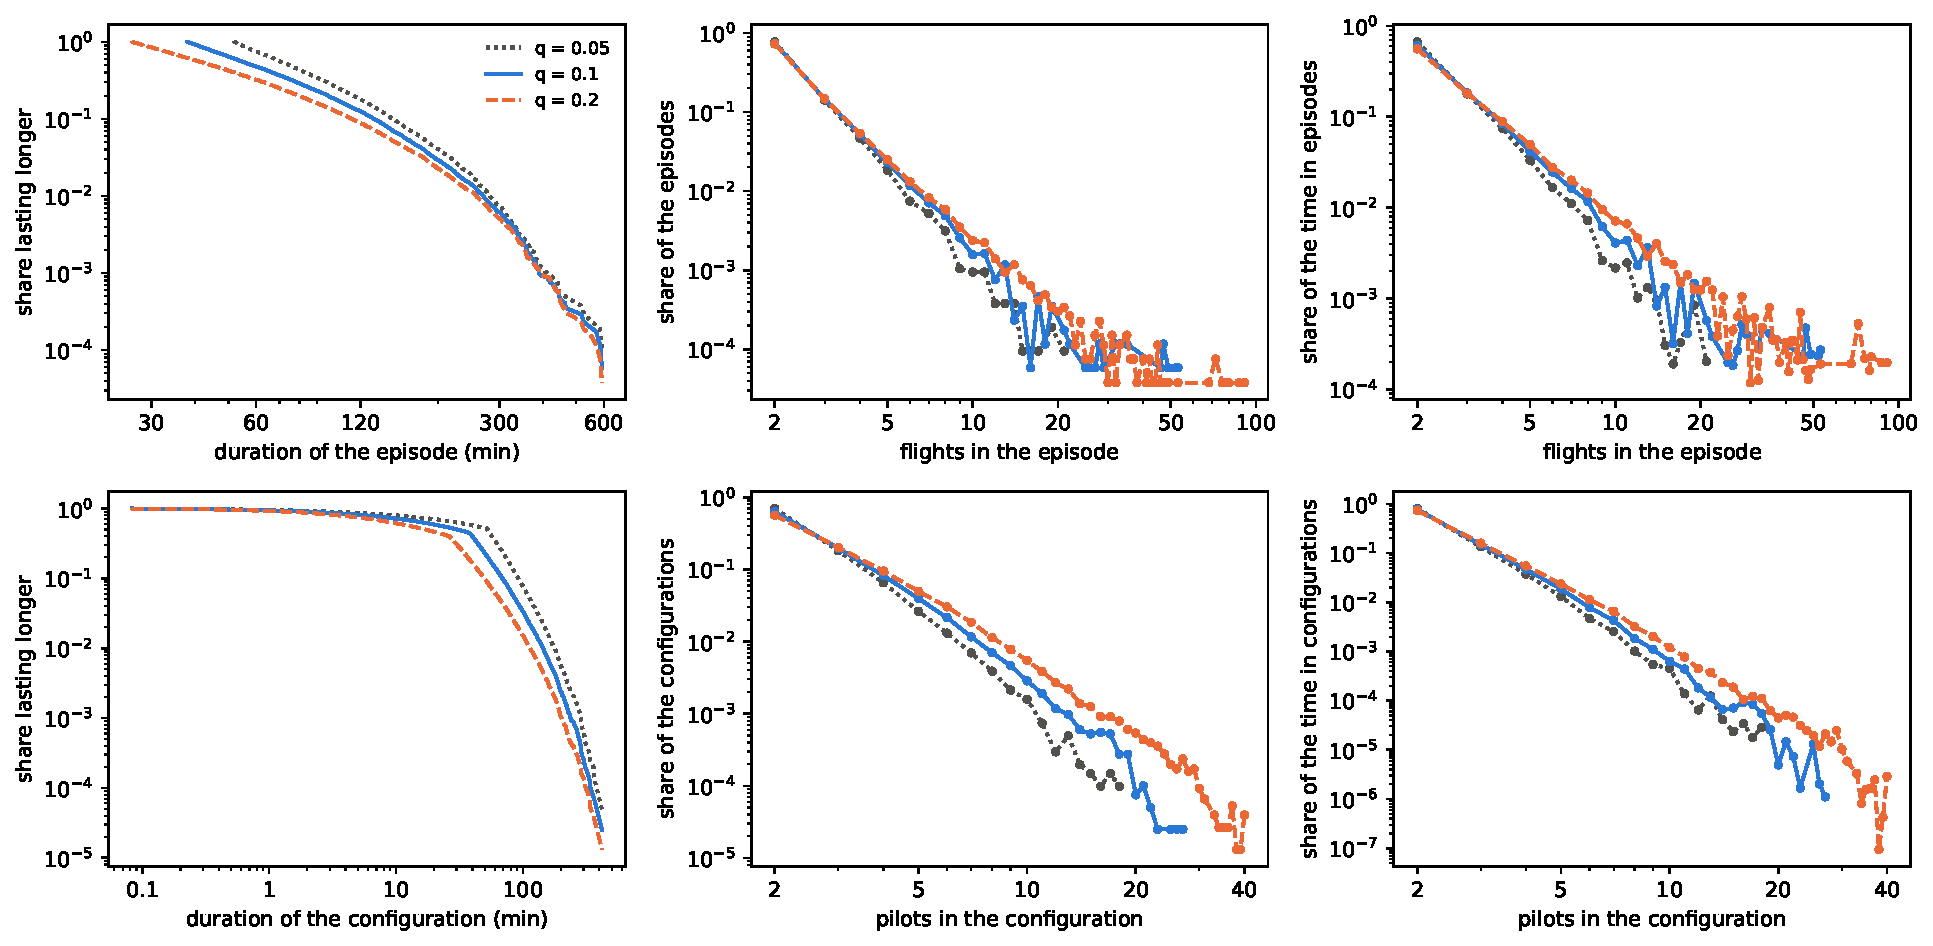
\includegraphics[width=\textwidth]{figures/assessment_structure.pdf}
\caption{Episodes (top) and configurations (bottom), $\delta=2$~min, whole archive, for three
values of $q$. Left: share lasting longer than a duration. Middle: share of each size. Right:
share of the total duration in each size.}
\label{fig:structure}
\end{figure}

\begin{table}
\centering
\small
\begin{tabular}{@{}l l r r c c c c r@{}}
\toprule
& $q$ & number & median & \multicolumn{2}{c}{2 participants} & \multicolumn{2}{c}{5 or more} & largest \\
& & & duration & items & time & items & time & \\
\midrule
episodes & 0.05 & 10\,553 & 74.6 min & 77\% & 67\% & 3.9\% & 8.1\% & 21 \\
 & 0.1 & 17\,169 & 58.2 min & 74\% & 61\% & 5.7\% & 12.6\% & 53 \\
 & 0.2 & 26\,504 & 44.5 min & 73\% & 56\% & 7.0\% & 17.2\% & 91 \\
\midrule
configurations & 0.05 & 20\,275 & 52.7 min & 70\% & 81\% & 5.6\% & 2.3\% & 18 \\
 & 0.1 & 40\,051 & 30.4 min & 63\% & 77\% & 9.4\% & 3.5\% & 27 \\
 & 0.2 & 75\,953 & 17.1 min & 56\% & 74\% & 14.1\% & 5.0\% & 40 \\
\bottomrule
\end{tabular}
\caption{Episodes and configurations for three values of $q$ ($\delta=2$~min). Items: share of
the episodes or configurations of that size; time: share of their total duration.}
\label{tab:structure}
\end{table}

With the chosen values the median episode lasts 58.2~min and three in four are pairs
(Table~\ref{tab:structure}). Episodes last at least $\tau^*$, since a contact must. Weighted by
duration the pairs weigh less, 61\% of the episode time, because larger episodes last longer:
those of five flights or more are 5.7\% of the episodes and 12.6\% of their time.

Configurations have no minimum duration: every arrival or departure of a member starts a new
one, so 10\% last less than 2.1~min, and the median is 30.4~min. Weighted by duration the pairs
weigh more, 77\% of the time against 63\% of the configurations, because large configurations
change quickly. \StWithHang\% of the configurations hold a hang glider.

A larger $q$, hence a shorter $\tau^*$, gives more and shorter groups, and larger ones: the
largest episode holds 21 flights with $q=0.05$, 53 with 0.1 and 91 with 0.2. The shares of the
small sizes change little; the tail moves.

\subsection{How configurations change}\label{sec:describe}

A configuration ends in one of five ways: a \emph{join} (members added), a \emph{leave} (members
removed in flight), a \emph{landing} (a removed member lands within 5~s, the grid step), a
\emph{split} (into several configurations) or a \emph{merge} (with others, into one); a
configuration of two pilots that loses one ends the group. Each ending is one component of a
bipartite graph between the configurations that end and those that start at one instant
(Appendix~\ref{app:graphs}). The rates are configurations ending per hour spent at each size
(Table~\ref{tab:rates}).

\begin{table}
\centering
\footnotesize
\begin{tabular}{@{}r r r l l l l l@{}}
\toprule
pilots & hours & median (min) & join & leave & landing & split & merge \\
\midrule
2 & 17\,389 & 41 & 0.31\,{\tiny[0.30, 0.32]} & 0.96\,{\tiny[0.95, 0.97]} & 0.098\,{\tiny[0.094, 0.10]} & -- & 0.085\,{\tiny[0.079, 0.092]} \\
3 & 3\,349 & 20 & 0.54\,{\tiny[0.52, 0.57]} & 1.6\,{\tiny[1.6, 1.6]} & 0.050\,{\tiny[0.044, 0.056]} & -- & 0.16\,{\tiny[0.15, 0.18]} \\
4 & 1\,059 & 13 & 0.70\,{\tiny[0.66, 0.76]} & 1.6\,{\tiny[1.6, 1.7]} & 0.042\,{\tiny[0.032, 0.051]} & 0.48\,{\tiny[0.45, 0.52]} & 0.26\,{\tiny[0.22, 0.29]} \\
5 & 421 & 11 & 0.88\,{\tiny[0.80, 0.96]} & 1.7\,{\tiny[1.6, 1.8]} & 0.036\,{\tiny[0.021, 0.057]} & 0.82\,{\tiny[0.76, 0.88]} & 0.32\,{\tiny[0.26, 0.37]} \\
6 & 176 & 8 & 1.1\,{\tiny[0.93, 1.2]} & 2.1\,{\tiny[1.9, 2.3]} & 0.028\,{\tiny[0.011, 0.048]} & 1.2\,{\tiny[1.0, 1.3]} & 0.51\,{\tiny[0.40, 0.63]} \\
7 & 96 & 7 & 1.1\,{\tiny[0.91, 1.3]} & 2.0\,{\tiny[1.8, 2.2]} & 0.031\,{\tiny[0.0089, 0.074]} & 1.3\,{\tiny[1.1, 1.5]} & 0.40\,{\tiny[0.30, 0.53]} \\
8+ & 107 & 4 & 1.8\,{\tiny[1.5, 2.2]} & 2.5\,{\tiny[2.2, 2.8]} & 0.028\,{\tiny[0.0084, 0.057]} & 2.7\,{\tiny[2.4, 3.1]} & 1.0\,{\tiny[0.73, 1.2]} \\
\bottomrule
\end{tabular}

\caption{By size: hours spent, median duration of a configuration, and configurations ending per
hour by outcome, with 5--95\% bands.}
\label{tab:rates}
\end{table}

\begin{itemize}
  \item \textbf{Most episodes never change:} \StEpisodeSingle\% of the \StEpisodes{} episodes are one
        configuration; \StEpisodeSplit\% hold a split, \StEpisodeMerge\% a merge.
  \item \textbf{The episode lasts, the configuration does not.} \StEpisodeTwoHours\% of the episodes
        last 2~h or more. A configuration lasts \StMedianConfTwo~min with 2 pilots and
        \StMedianConfMax~min with \StSizeMax{} or more: joins, leaves, splits and merges all grow with
        size, so a large configuration changes members every few minutes.
  \item \textbf{Groups break in flight:} \StEndFlight\% of the \StEnds{} configurations that end a group
        do so in flight, \StEndLanding\% at a landing. \StFormDeparture\% of the \StFormations{}
        configurations with no predecessor form when a member departs: pilots who took off together.
  \item \textbf{A pair} ends \StRateLeaveTwo{} times per hour because the two separate, \StRateJoinTwo{}
        because a third pilot joins, \StRateMergeTwo{} by a merge and \StRateLandingTwo{} by a landing.
\end{itemize}

\subsection{Where in the flight groups form and break}\label{sec:phases}

On 1~Hz flights, where the phases are labelled: the phase at the instant a flight enters
(\Entries{}) or leaves (\Exits{}) a group, against the shares of time in each phase; entries at the
departure (\AtDeparture{}) and exits at the landing (\AtLanding{}) are counted apart
(Figure~\ref{fig:phases}, Table~\ref{tab:phases}).

\begin{figure}
\centering
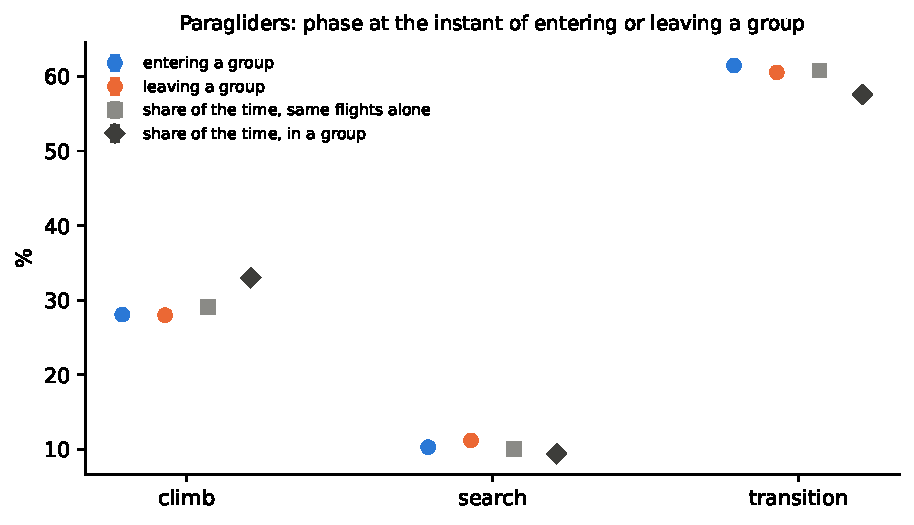
\includegraphics[width=0.55\textwidth]{figures/structure/mechanisms_phases.pdf}
\caption{Phase at entry and exit, against the time shares (bands: blocks).}
\label{fig:phases}
\end{figure}

\begin{table}
\centering
\footnotesize
\begin{tabular}{@{}l l l l@{}}
\toprule
 & climb (\%) & search (\%) & transition (\%) \\
\midrule
entering a group & 28.1 [27.6, 28.5] & 10.3 [10.0, 10.6] & 61.5 [61.0, 61.9] \\
leaving a group & 28.0 [27.6, 28.3] & 11.2 [10.9, 11.5] & 60.6 [60.1, 61.0] \\
share of time, alone & 29.1 [28.9, 29.3] & 10.1 [10.0, 10.2] & 60.8 [60.6, 61.0] \\
share of time, in a group & 33.0 [32.8, 33.2] & 9.4 [9.2, 9.6] & 57.6 [57.3, 57.9] \\
\bottomrule
\end{tabular}

\caption{Phase at the instant of entering or leaving a group, and shares of time in each phase
(percent, with 5--95\% bands; 1~Hz flights).}
\label{tab:phases}
\end{table}

Entries fall in climbs \PhaseEntryClimb\%, searches \PhaseEntrySearch\% and glides
\PhaseEntryTransition\% of the cases, exits \PhaseExitClimb, \PhaseExitSearch, \PhaseExitTransition\%,
against \PhaseAloneClimb, \PhaseAloneSearch, \PhaseAloneTransition\% of the time alone: there is no
phase where groups preferentially form or break. \EntriesEarly\% of the entries are within 10~min of
the departure.

\subsection{When in the day}\label{sec:hours}

\begin{figure}
\centering
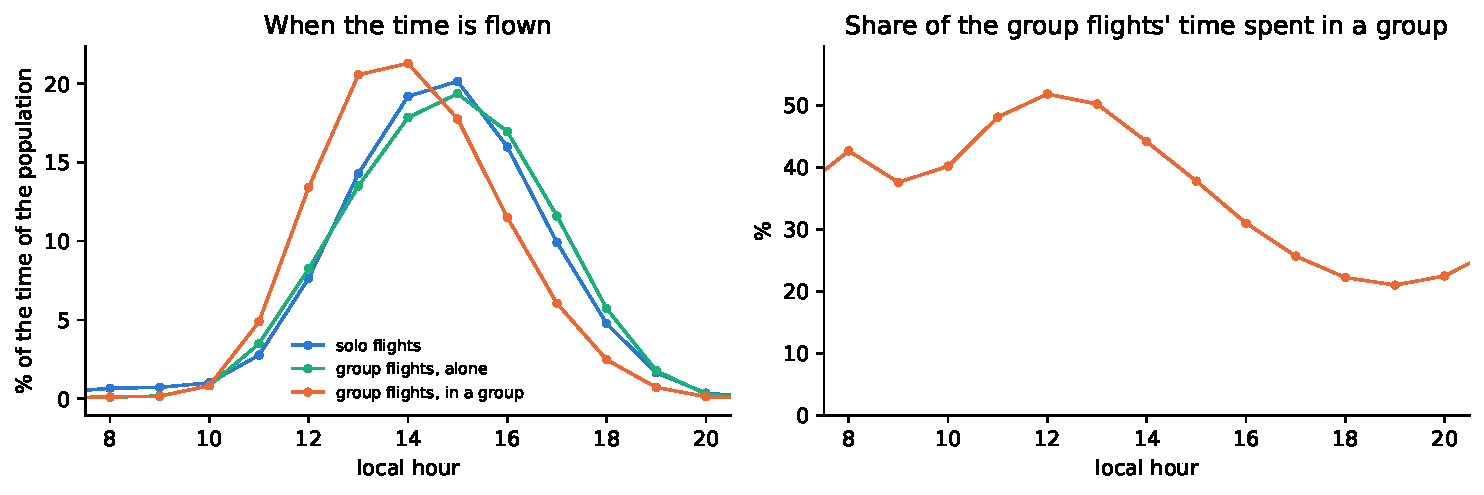
\includegraphics[width=0.9\textwidth]{figures/structure/mechanisms_hours.pdf}
\caption{Time of solo flights (S), of group flights alone (A) and in a group (G) over the local hour
(left), and the share of a group flight's time spent in a group (right).}
\label{fig:hours}
\end{figure}

Group time is concentrated around midday: \GroupShareNoon\% of a group flight's time at
\GroupShareNoonHour~h, \GroupShareMorning\% at 9~h, \GroupShareEvening\% at 18~h
(Figure~\ref{fig:hours}).
